\begin{figure}[htbp]
\centering
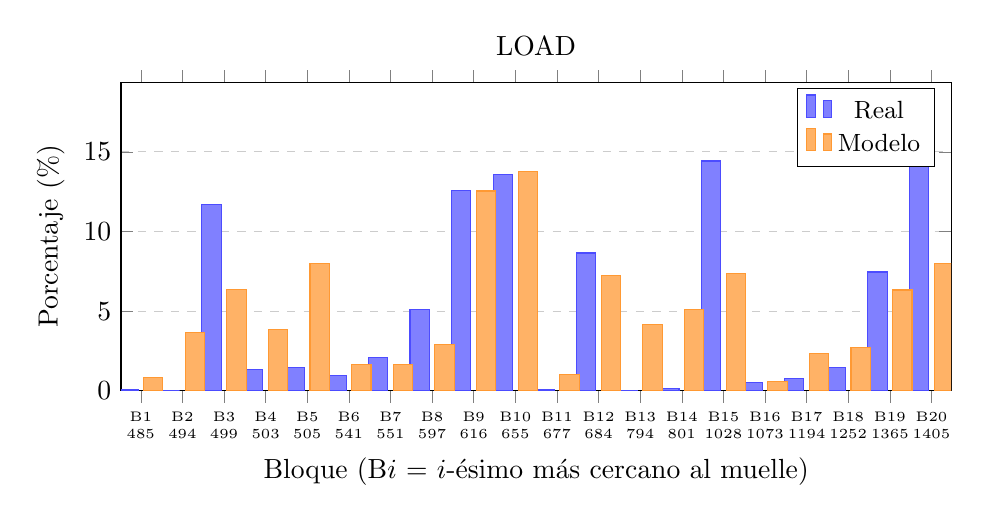
\begin{tikzpicture}
\begin{axis}[
  ybar, bar width=7pt, width=\textwidth, height=5.5cm,
  title={LOAD},
  xlabel={Bloque (B$i$ = $i$-ésimo más cercano al muelle)},
  ylabel={Porcentaje (\%)},
  xtick={0,1,2,3,4,5,6,7,8,9,10,11,12,13,14,15,16,17,18,19},
  xticklabels={{B1\\485},{B2\\494},{B3\\499},{B4\\503},{B5\\505},{B6\\541},{B7\\551},{B8\\597},{B9\\616},{B10\\655},{B11\\677},{B12\\684},{B13\\794},{B14\\801},{B15\\1028},{B16\\1073},{B17\\1194},{B18\\1252},{B19\\1365},{B20\\1405}},
  xticklabel style={font=\tiny, align=center},
  ymin=0,
  legend style={at={(0.98,0.98)}, anchor=north east, font=\small},
  ymajorgrids=true, grid style={dashed,gray!40},
  enlarge x limits=0.025,
]
\addplot[fill=blue!50, draw=blue!70] coordinates {(0,0.10) (1,0.00) (2,11.70) (3,1.31) (4,1.45) (5,0.95) (6,2.07) (7,5.10) (8,12.56) (9,13.61) (10,0.07) (11,8.65) (12,0.03) (13,0.16) (14,14.43) (15,0.53) (16,0.76) (17,1.45) (18,7.46) (19,17.62)};
\addplot[fill=orange!60, draw=orange!80] coordinates {(0,0.83) (1,3.65) (2,6.36) (3,3.83) (4,8.00) (5,1.67) (6,1.64) (7,2.88) (8,12.55) (9,13.78) (10,1.01) (11,7.22) (12,4.14) (13,5.12) (14,7.34) (15,0.60) (16,2.33) (17,2.71) (18,6.33) (19,8.00)};
\legend{Real, Modelo}
\end{axis}
\end{tikzpicture}
\vspace{4pt}
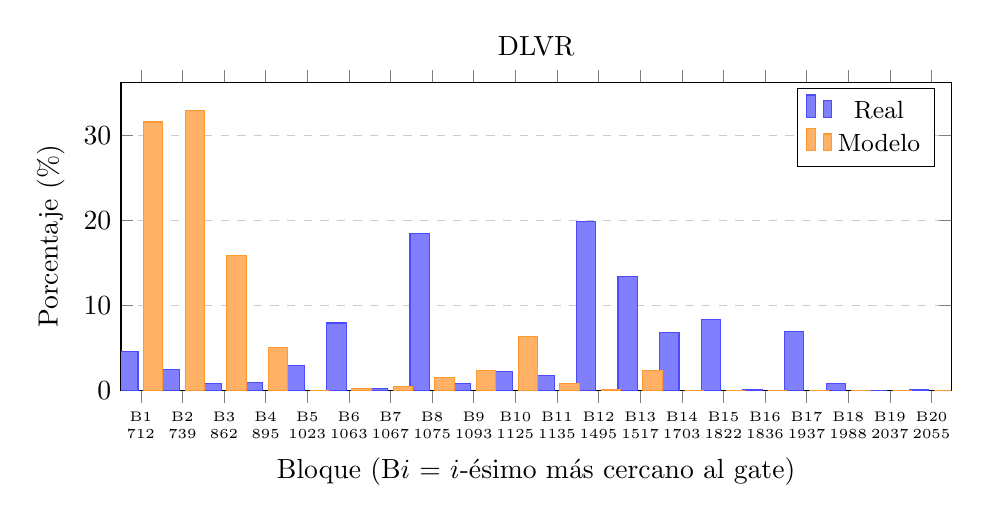
\begin{tikzpicture}
\begin{axis}[
  ybar, bar width=7pt, width=\textwidth, height=5.5cm,
  title={DLVR},
  xlabel={Bloque (B$i$ = $i$-ésimo más cercano al gate)},
  ylabel={Porcentaje (\%)},
  xtick={0,1,2,3,4,5,6,7,8,9,10,11,12,13,14,15,16,17,18,19},
  xticklabels={{B1\\712},{B2\\739},{B3\\862},{B4\\895},{B5\\1023},{B6\\1063},{B7\\1067},{B8\\1075},{B9\\1093},{B10\\1125},{B11\\1135},{B12\\1495},{B13\\1517},{B14\\1703},{B15\\1822},{B16\\1836},{B17\\1937},{B18\\1988},{B19\\2037},{B20\\2055}},
  xticklabel style={font=\tiny, align=center},
  ymin=0,
  legend style={at={(0.98,0.98)}, anchor=north east, font=\small},
  ymajorgrids=true, grid style={dashed,gray!40},
  enlarge x limits=0.025,
]
\addplot[fill=blue!50, draw=blue!70] coordinates {(0,4.57) (1,2.54) (2,0.85) (3,0.96) (4,2.94) (5,7.96) (6,0.21) (7,18.48) (8,0.83) (9,2.22) (10,1.82) (11,19.84) (12,13.40) (13,6.89) (14,8.41) (15,0.19) (16,7.00) (17,0.80) (18,0.00) (19,0.11)};
\addplot[fill=orange!60, draw=orange!80] coordinates {(0,31.57) (1,32.95) (2,15.92) (3,5.13) (4,0.00) (5,0.27) (6,0.49) (7,1.60) (8,2.39) (9,6.33) (10,0.81) (11,0.15) (12,2.39) (13,0.00) (14,0.00) (15,0.00) (16,0.00) (17,0.00) (18,0.00) (19,0.00)};
\legend{Real, Modelo}
\end{axis}
\end{tikzpicture}
\caption{Distribución porcentual de flujos por bloque, semana~3 (2022-01-17). Bloques ordenados por distancia creciente al destino. Barras azules: operación real; barras naranjas: modelo.}
\label{fig:flujos-sem3}
\end{figure}